
%(BEGIN_QUESTION)
% Copyright 2008, Tony R. Kuphaldt, released under the Creative Commons Attribution License (v 1.0)
% This means you may do almost anything with this work of mine, so long as you give me proper credit

Small relays often come packaged in clear, rectangular, plastic cases.  These so-called ``ice cube'' relays have either eight or eleven pins protruding from the bottom, allowing them to be plugged into a special socket for connection with wires in a circuit:

$$
\includegraphics[width=15.5cm]{i03165x01.eps}$$

Draw the necessary connecting wires between terminals in this circuit, so that actuating the normally-open pushbutton switch will energize the relay, which will in turn supply electrical power to the motor.  The pushbutton switch should not carry any motor current, just enough current to energize the relay coil:

$$\includegraphics[width=15.5cm]{i03165x02.eps}$$

\underbar{file i03165}
%(END_QUESTION)





%(BEGIN_ANSWER)

This is a graded question -- no answers or hints given!

%(END_ANSWER)





%(BEGIN_NOTES)

This is by no means the only solution, but it works:

$$\includegraphics[width=15.5cm]{i03165x03.eps}$$

A common source of trouble for students when sketching this circuit is how to ensure only the relay contacts (and not the pushbutton switch) carries the motor's current.  

\vskip 10pt

One way to help understand how to wire the circuit is to {\it sketch a schematic diagram} of what you wish to build, before attempting to connect the points in the pictorial diagram.  This strategy works by separating what are really two different problems: (1) how to wire any relay so that the contacts alone carry load current, and (2) how to connect the terminals in this particular circuit the way you need them to implement the desired function.  Take the following schematic diagram as an example, seeing how much easier it is to interpret than the pictorial sketch:

$$\includegraphics[width=15.5cm]{i03165x04.eps}$$

%INDEX% Pictorial circuit review (relay circuit)

%(END_NOTES)


